\documentclass[12pt,a4paper,oneside]{article}
\usepackage[utf8]{inputenc}
\usepackage[english]{babel}
\usepackage{amsmath}
\usepackage{amsfonts}
\usepackage{amssymb}
\usepackage[left=1cm,right=1cm,top=1cm,bottom=1cm]{geometry}
\usepackage{graphicx}
\usepackage{hyperref}
\usepackage{multicol}
\renewcommand{\familydefault}{garamond}
\begin{document}

\pagenumbering{gobble}

\begin{center}
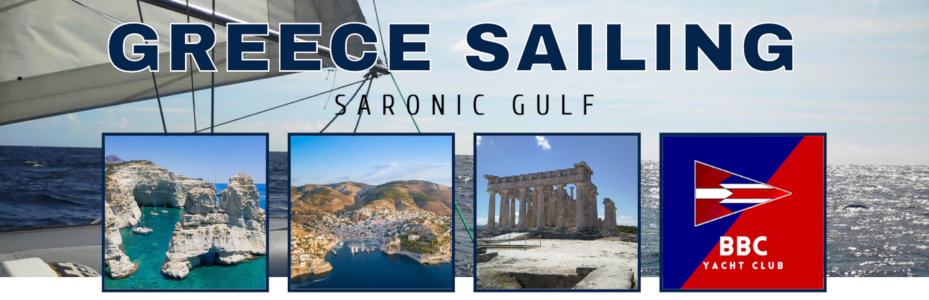
\includegraphics[scale=0.5]{../images/saronic_header_small.png} \\
{\Large \textsc{Day 1 - 31/09/2023 : $\Upsilon\delta\rho\alpha$ (Hydra/Idra), Saronic Gulf}}
\line(1,0){450}
\end{center}

\begin{multicols}{2}

\subsection*{Location}
\begin{tabular}{l|r}
Lat: & 35° 48' 32" N \\  
Long: & 008° 58' 22" E \\ 
\end{tabular} 

\noindent 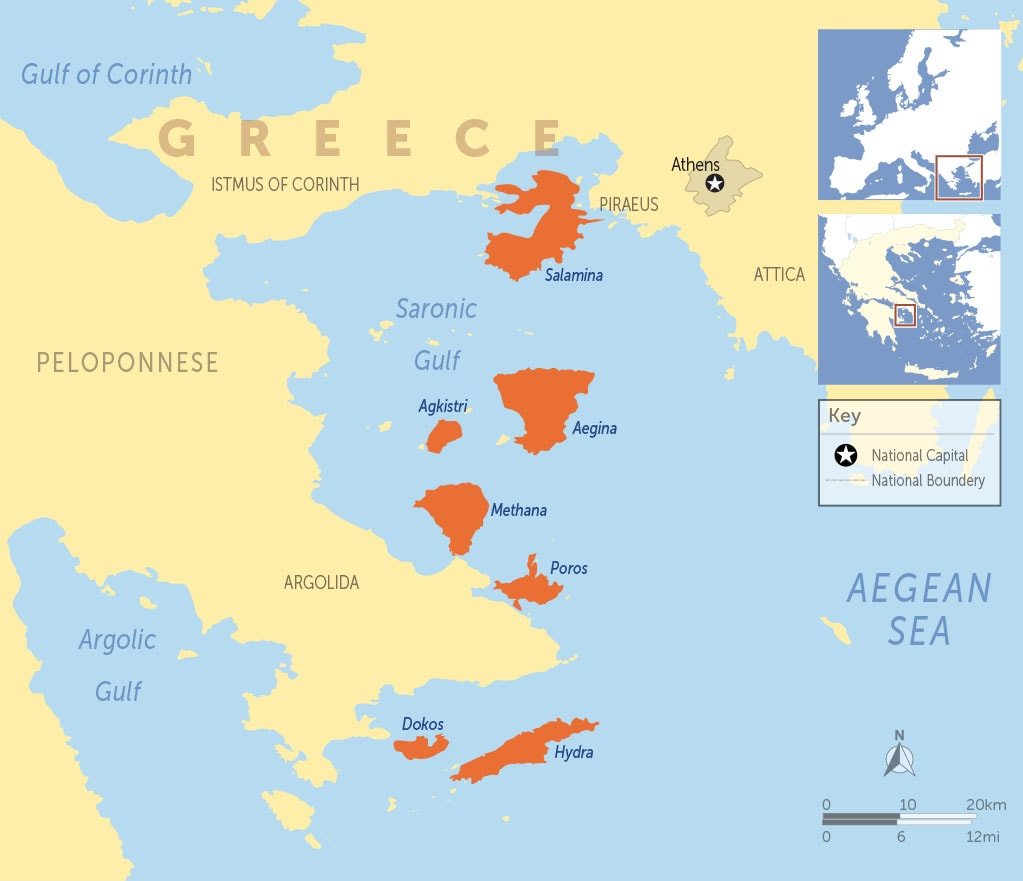
\includegraphics[scale=0.25]{saronic-map.jpg} 

\subsection*{Weather}
\noindent \textbf{Saronic Gulf}\\
North 3 or 4 soon. Up to slight. Locally poor. Chance of Rain\\

\noindent \textbf{SW Aegean}\\
North 3 or 4 soon variable. Slight. Locally poor. Chance of Rain\\

\subsection*{Important - Before Leaving}

Water is in short supply on island and may be unavailable for visitors, fill up before arriving.

\subsection*{Almanac}
\begin{tabular}{p{2cm} p{2cm} p{3cm}}
Sunrise: 05:42 & Sunset: 19:34 &	Age of Pisces\\
Moonrise: 18:34 & Moonset: 04:35 & Moon Illumination: 56\% \\
\end{tabular}

\noindent Stars and Constellations:

\subsection*{Destination}

There is one main town, known simply as "Hydra port" (pop. 1,900 in 2011). It consists of a crescent-shaped harbor, around which is centered a strand of restaurants, shops, markets, and galleries that cater to tourists and locals (Hydriots). Steep stone streets lead up and outward from the harbor area.

The name Hydra comes from ancient Greek $\Upsilon\delta\rho\alpha$ (hydra), derived from the Greek word for "water", a reference to the natural springs on the island.

By law, cars and motorcycles are not allowed. Horses, mules and donkeys, and water taxis provide public transportation.

In 2007, a National Geographic Traveler panel of 522 experts rated Hydra the highest of any Greek island (11th out of 111 islands worldwide), as a unique destination preserving its "integrity of place".

In the 19th century, Hydra was home to some 125 boats and 10,000 sailors. The mansions of the sea captains that ring the harbor are a testament to the prosperity that shipping brought to the island, which, at the time of the Greek Revolution, had 16,000 inhabitants

In the 1950s and 1960s Hydra was the adopted home of a community of expatriate artists that included celebrated Norwegian novelist Axel Jensen, Australian writers Charmian Clift and George Johnston, and Canadian singer-songwriter Leonard Cohen.

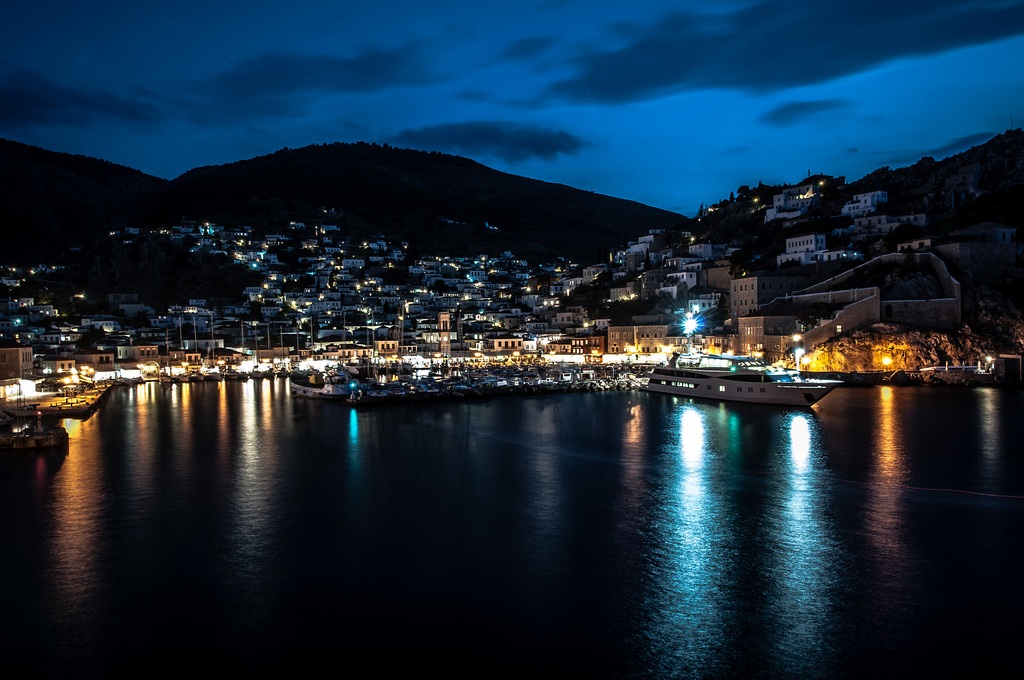
\includegraphics[scale=0.24]{hydra-visualhunt.jpg} 

Although the island's name is derived from ancient springs known to the Ancient Greeks, it is now almost dry. Hydra previously had wells, and three new wells have been found. Today, the island imports its water by boat from the Greek mainland. A new desalinization plant has been finished but is not in operation. 

\subsection*{Pilotage and Navigation}

Arrival Waypoint: 4-10\\

Hydra Port is small and busy. Pilot book suggests arriving by 2pm. Even then, you may need to raft Mediterranean style - Make sure you only drop your anchor directly opposite where you will raft, reverse slowly and tie stern between the bows of 2 boats. Use plank of wood to walk between boats and shore. Have a snorkeller ready when departing - you may need to disentangle.

Water is in short supply on island, fill up before arriving.

\subsection*{Evening Information}

Hydra is a popular destination for wealthy Athenians and as such, waterfront premises are expensive (pilot book describes them as Manhattan prices).  

We have a restaurant booked for all 4 boat crews at 19:00.

\subsection*{Links}
\begin{tabular}{p{7cm}}
\url{https://en.wikipedia.org/wiki/Hydra_(island)} \\ 
\url{https://www.theguardian.com/travel/2020/may/23/hydra-the-greek-island-for-dreamers}\\ 
\end{tabular} 

\end{multicols}

\noindent Simon Thompson\\
BBCYC Greek Naviguesser
\end{document}